\chapter{Evaluation} \label{chap:evaluation}

In the previous chapter, \S\ref{chap:system}, we have presented our implementation of live migration of containers using \criu and \runc, and have motivated our design choices with micro-benchmarks that fulfil the initial objectives specified in the introduction.
In this chapter, we move on to evaluate the system as a whole, and how the different features interlace and work together, and  how does our system compare to traditional virtual machine live migration.

In all the experiments here presented, and unless otherwise stated, we use the same experimental setup than in the micro-benchmark chapter.
Two (if necessary) Linux Debian machines with kernel version $4.19.0-6$ running on a host-only network in VirtualBox version $5.2.34$.
\criu version $3.13$ and \runc version $1.0.0-rc8$, both built from source.

\section{Application Downtime}

\cs{Re-do the initial plot presented}

\cs{Include the content from Decentralized Systems}

\section{Memory Scalability}

In this section we study the scalability of our approach with respect to the memory allocated by the to-be checkpointed container.
For this experiment we set up a \textsc{Redis} in-memory database which we pre-load with a variable number of key-value pairs.
We use \texttt{redis-client} and \texttt{redis-server} version $5.0.3$, and pre-load the keys using 

\begin{figure}[h!]
    \centering
    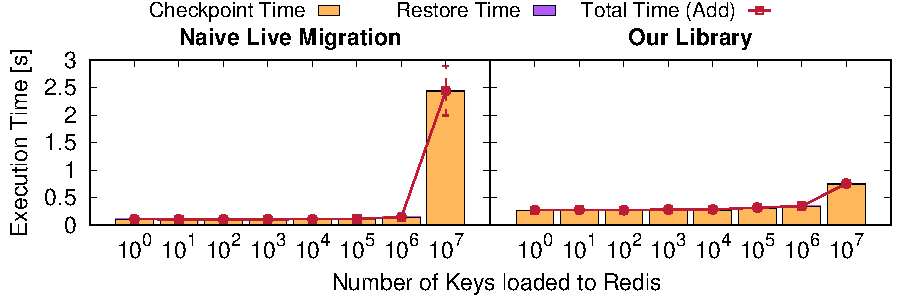
\includegraphics[width=\textwidth]{figs/key-scalability/key_scalability.pdf}
    \caption[Scalability with respect to the memory to transfer.]{Scalability with respect to the memory to transfer. We compare our system with manual live migration when running in the same machine with a one-shot migration.\label{fig:key-scalability}}
\end{figure}

\cs{Downtime as we increase the number of iterations (i.e. threshold)}

\cs{Comparison with VM Teleport}

\begin{lstlisting}[style=Bash,caption={Script to teleport a VirtualBox VM, and run the macrobenchmark.},label={code:vm-teleport}]
#!/bin/bash

# Configure target machine to wait for a teleport request to arrive
VBoxManage modifyvm 'CRIU-Debian-Teleport-Target' --teleporter on --teleporterport 6000

# Iterate over the different number of keys
for num_keys in 1 10 100 1000 10000 100000 1000000 10000000
do
    # Start the host machine as usual
    ssh <HOST_VM>
    cd ~/runc-containers/redis && ./run_redis.sh 100000

    # Start the target machine, if using a normal start, a process dialog will appear

    # Run the migration
    time VBoxManage controlvm 'CRIU-Debian' teleport --host localhost --port 6000

    # Shut down both VMs
done
\end{lstlisting}

\begin{figure}[h!]
    \centering
    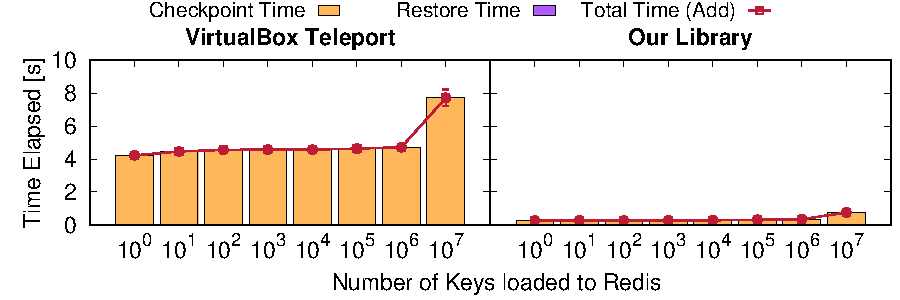
\includegraphics[width=\textwidth]{figs/vm-teleport/vm_teleport.pdf}
    \caption[Scalability comparison with VirtualBox Teleport.]{Scalability with respect to the memory to transfer. We compare our system with VM live migration using VirtualBox's Teleport functionality.\label{fig:vm-teleport}}
\end{figure}

\cs{Compare with P-Haul if time}
